\documentclass[conference]{IEEEtran}

% correct bad hyphenation here
%\hyphenation{op-tical net-works semi-conduc-tor}
\newcommand{\ENABLECOMMENTS}{}
\usepackage{listings}
\usepackage{ifpdf}
\usepackage{wrapfig}
\usepackage{url}
\usepackage{subcaption}
\ifpdf
\usepackage[pdftex]{graphicx}
\else
\usepackage{graphicx}
\fi
\newcommand{\iap}{\textit{DREMS}\ }
%\newcommand{\iapfull}{\textbf{D}istributed \textbf{S}oftware \textbf{P}latform }
\newcommand{\iapfull}{\textbf{D}istributed \textbf{RE}altime \textbf{M}anaged \textbf{S}ystem}


\usepackage{color}

\usepackage{tikz}
\usetikzlibrary{matrix,arrows,circuits.ee,circuits.ee.IEC,shapes.geometric,shapes.misc}
\ifdefined\ENABLECOMMENTS
\newcommand{\comment}[2]{{\texttt{\color{red}#1:#2}}}
\else
\newcommand{\comment}[2]{}
\fi

\begin{document}
%
% paper title
% can use linebreaks \\ within to get better formatting as desired
\title{ROSMOD: A Toolsuite for Modeling, Generating, Deploying, and Managing Distributed Real-time Component-based Software using ROS}


% author names and affiliations
% use a multiple column layout for up to three different
% affiliations
\author{\IEEEauthorblockN{Pranav Srinivas Kumar, William Emfinger, \\
Amogh Kulkarni and Gabor Karsai\IEEEauthorrefmark{1}}
\IEEEauthorblockA{\IEEEauthorrefmark{1}
Institute for Software Integrated Systems,\\ Electrical Engineering and Computer Science, Vanderbilt University,\\
%  1025 16th Ave S, \\
Nashville, TN 37235, USA \\
Email:\{pkumar, emfinger, kulkaras, gabor\}@isis.vanderbilt.edu}
\and
\IEEEauthorblockN{Dexter Watkins, Benjamin Gasser, \\ 
Cameron Ridgewell and Amrutur Anilkumar\IEEEauthorrefmark{2}}
\IEEEauthorblockA{\IEEEauthorrefmark{2}
Mechanical Engineering, Vanderbilt University\\
Nashville, TN 37235, USA \\
Email:\{dexter.a.watkins, benjamin.w.gasser, \\ cameron.p.ridgewell, amrutur.v.anilkumar\}@vanderbilt.edu}
}


% make the title area
\maketitle

\begin{abstract}
%We have created a testbed for the development and testing of Cyber-Physical Systems (CPS) applications.  This testbed incorporates smart network hardware which allows for high-fidelity emulation of the system's network characteristics, and simulation systems which allow for high-fidelity simulation of the CPS, its environment, its sensors, and its actuators.  We discuss the architecture of this testbed, the types of experiments and applications which can be run on the testbed, some of the testbed's limitations, and some extensions to the testbed. 

This paper describes a testbed for development, deployment, testing, and analysis of Cyber-Physical Systems (CPS) applications. The testbed incorporates smart network hardware, allowing high-fidelity emulation of CPS network characteristics, and CPS simulation environments to enable high-frequency sensor reading, actuator control and physical environmental changes. We discuss the architecture of this testbed and present the types of experiments and applications which can be run to study hardware and software fault tolerance, software reconfiguration, and system stability characteristics in distributed real-time embedded systems. We also describe the scalability, limitations, and potential extensions to this testbed.
\end{abstract}
\section{Introduction}

% What is ROS?
Robot Operating System (ROS) \cite{ROS} is a meta-operating system framework that facilitates robotic system development. ROS is widely used in various fields of robotics including industrial robotics, UAV swarms and low-power image processing devices. The open source multi-platform support of ROS has made it a requirement in several DARPA robotics projects including the \emph{DARPA Robotics Challenge} \cite{DARPA_Robotics_Challenge}.   

% What does ROS provide
ROS enables the deployment of a network of interacting ROS \emph{nodes}, that communicate using the ROS middleware infrastructure. ROS nodes can contact each other using different types of interaction patterns including synchronous remote method invocation (RMI) and asynchronous message passing publish-subscribe interactions. A ROS application is a packaged set of ROS nodes that communicate through a ROS Master, where a ROS Master is a single discovery and communications broker that facilitates node-node flow setup.

% What is ROSMOD
This paper describes ROSMOD \cite{ROSMOD}, an open source development tool suite and run-time software platform for rapid prototyping component-based software applications using ROS. Using ROSMOD, an application developer can create, deploy and manage ROS applications for distributed real-time embedded systems. We define a strict component model, a model-driven development workflow and run-time management tools to build and deploy component-based software with ROS. 

% AGSE - Tell readers about how ROSMOD is used
The utility of ROSMOD is described using a real-world case study - An Autonomous Ground Support Equipment (AGSE) robot that was designed, prototyped and deployed for the NASA Student Launch Competition \cite{NASA_SL} 2014-2015. We describe the challenges and requirements, the robotic design, the software prototyping and the overall performance that lead us to winning this competition.

% Following sections 
The sections in this paper are organized as follows. Section \ref{sec:ROSMOD} describes the ROSMOD tool suite: The component model, modeling language, graphical user interface, code generators and deployment infrastructure. Section \ref{sec:Case_Study} describes our AGSE robot and evaluates ROSMOD. Section \ref{sec:Future_Work} describes our current efforts to improving ROSMOD support with analysis tools and run-time reconfiguration solutions. Section \ref{sec:Related_Research} presents related efforts in the field of robotics, both using ROS and other similar middleware platforms. Finally, Section \ref{sec:Conclusions} presents concluding remarks.

\section{ROSMOD Tool Suite}
\label{sec:ROSMOD}

\subsection{Component Model}

Software development using ROSMOD is influenced by the principles of Component-based Software Engineering
\cite{CBSE}\cite{Heineman:01}. Large and complex systems are built by assembling reusable software pieces called \emph{components}. ROSMOD Components contain executable code that implement functions, manipulate state variables and interact with other components in the applications. This model is inspired by our previous efforts with the F6COM Component Model \cite{DREMS_CM}. The architecture of a ROSMOD component is shown in Figure \ref{fig:ROSMOD_Component}.

ROSMOD components can contain (1) publishers, (2) subscribers, (3) clients, (4) servers and (5) timers. Publisher ports publish (without blocking) messages of a message topic, and Subscriber ports subscribe to a message topic. Client ports require the services offered by server ports. Server ports provide services that can be used by the external world. Lastly, periodic and sporadic timers are used to trigger components. The semantics of these communication patterns are dictated by ROS.

To facilitate interactions with other components in an ordered manner, each component has a \emph{Component Message Queue}. This queue holds requests (i.e. messages) received from other interacting components or from the component's timers. %This queue supports a variety of scheduling schemes such as FIFO (first-in-first-out), PFIFO (priority-FIFO) and EDF (earliest-deadline-first) to enqueue received requests. 
These requests are processed by a single thread (per component) called the \emph{Component Executor Thread}. This thread is therefore responsible for executing all triggered callbacks e.g. subscriber callbacks, server callbacks and timer callbacks. 

\begin{figure}[h]
	\centering
	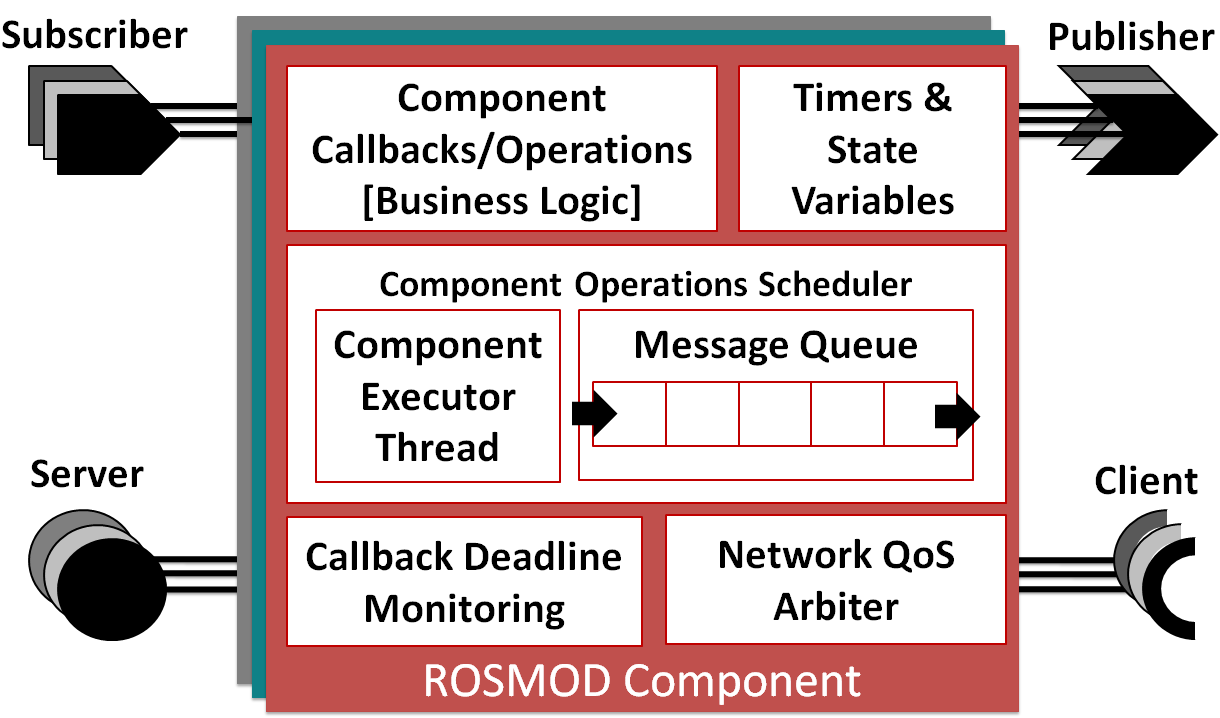
\includegraphics[width=0.45\textwidth]{figs/ROSMOD_Component.png}
	\caption{ROSMOD Component}
	\label{fig:ROSMOD_Component}
\end{figure}

\vspace{-0.1in}

Figure \ref{fig:Component_Message_Queue} shows a simple Client-Server component interaction. An Image Processor component is periodically triggered by a timer. At each timer expiry, this component, using its client port, makes a blocking remote procedure call to a Camera component. This service request is enqueued onto the Camera's message queue, and, when it reaches the front of the queue, the Camera component executor thread executes the corresponding server callback, returning the response to the Image Processor. This message queue-based interaction is also true for timers; when the timer in the Image Processor expires, a timer callback request is enqueued onto its message queue and eventually processed. 

\begin{figure}[h]
	\centering
	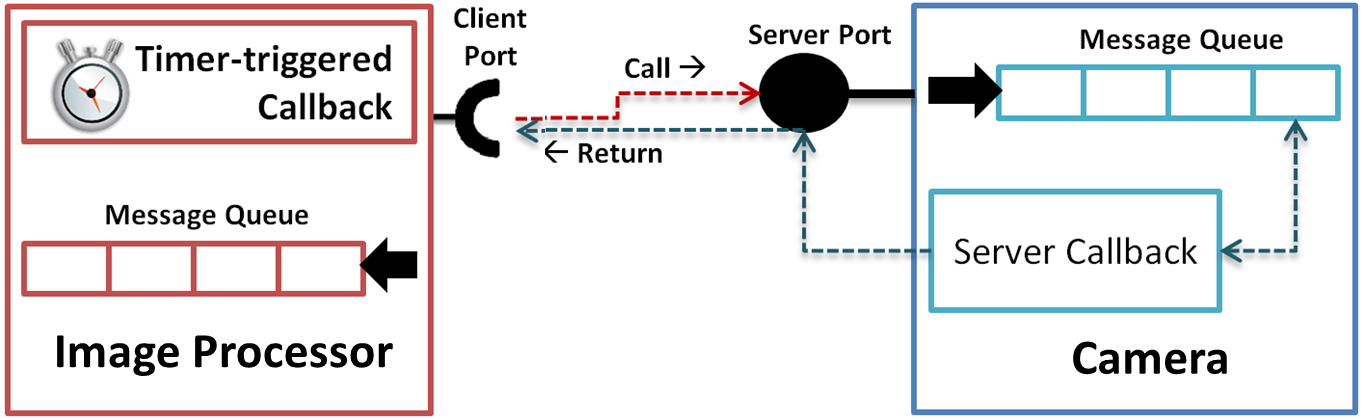
\includegraphics[width=0.48\textwidth]{figs/Component_Message_Queue.png}
	\caption{Component Interactions}
	\label{fig:Component_Message_Queue}
\end{figure}

It must be noted here that in each component, the message queue is processed by a single executor thread. Multiple components may run concurrently but each component's execution is single-threaded. Also, the component message queue supports several scheduling schemes including FIFO (first-in first-out), PFIFO (priority first-in first-out) and EDF (earliest deadline first). Requests in the message queue are processed using a non-preemptive scheduling scheme. This means that each callback/operation run by the executor thread is run to completion before the next one (waiting in the message queue) is processed. These rules are strictly applied to all ROSMOD components.

The single-threaded component execution is an important choice as it allows robust application development that is free of race conditions. Application integrators can avoid using synchronization primitives and locking mechanisms while developing code and this greatly simplifies design. These choices also more easily enable support for non-functional properties such as fault isolation and tolerance, operation timeliness and component lifecycle management. 

% ROS client library implementation called rosmod

\subsection{Modeling Language}

ROSMOD Projects are built using the ROSMOD Modeling Language. With this language, ROS users can create models of ROS workspaces, hardware topologies, deployment plans and more. The tool suite provides a Graphical User Interface to build these models but the state and configuration properties of the project are saved in a set of text files (models) that follow a strict set of grammatical rules, written using Antlr 4 \cite{ANTLR_BOOK}. Figure \ref{fig:ROSMOD_Project} shows the metamodel of the textual modeling language as a UML \cite{UML} class diagram.

\begin{figure*}[t]
	\centering	
	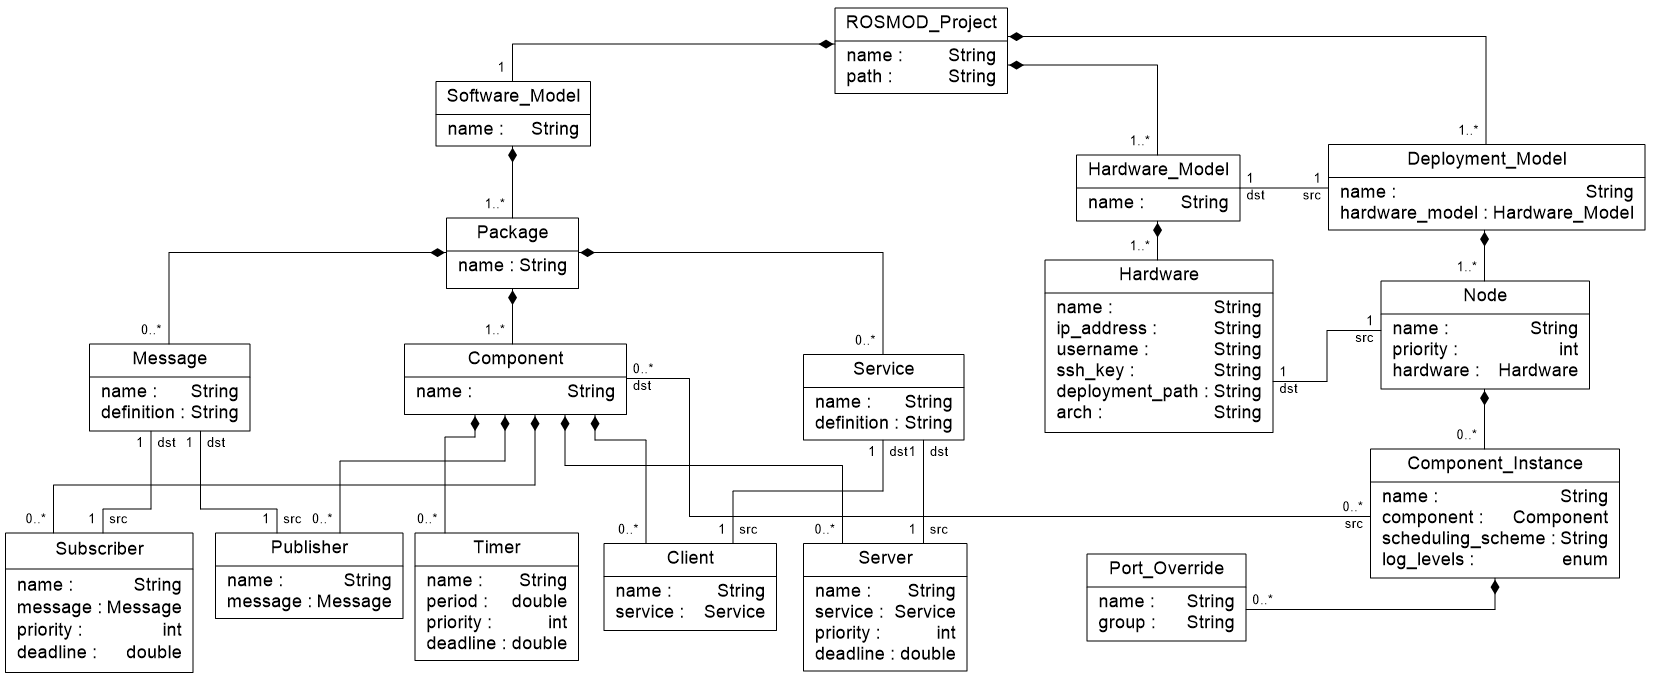
\includegraphics[width=1.0\linewidth]{figs/ROSMOD_Project.png}
	\caption{ROSMOD Project}
	\label{fig:ROSMOD_Project}	
\end{figure*}

\subsubsection{ROS Background}
ROS workspaces are high-level containers for source code which may contain one or more ROS packages.  ROS packages are containers which may include (1) one or more ROS message definitions for asynchronous publish/subscribe, (2) one or more ROS service definitions for synchronous RMI, and (3) one or more ROS Nodes, which are processes that can communicate with each other using predefined ROS messages or ROS services.  In this way a ROS package can be thought of as an application, and a ROS node is a process in that application.

\subsubsection{Software Model}
The ROSMOD Software model represents a ROS workspace. Each model consists of one or more ROS packages. Each ROS package contains definitions to (1) messages, (2) services and (3) components. The component assembly is derived from the interacting component ports. Ports that are associated with callbacks e.g. subscribers, contain both a \emph{priority} and a \emph{deadline} property to facilitate the scheduling schemes in the component model.

\subsubsection{Hardware Model}

Hardware models completely describe the hardware architecture of the system. Here, the user describes the different hardware hosts available for deployment, including their properties such as IP address, username and SSH keys.  These properties allow the user to directly map executables to hardware in a specified network and allow the deployment infrastructure to manage all remote operations and help ensure security between applications.  Deployment models refer to such predefined hardware models when mapping processes to hardware devices. Current work aims to improve on this hardware model by adding concepts for subnets, network interface controllers (NIC) and network links between hardware devices to more accurately represent the network topology.

\subsubsection{Deployment Model}

ROSMOD Deployment models contain the specifications for ROS nodes (executable processes). Each ROS node is ranked by a process priority and is mapped to a specific hardware device on which it will be executed. Each ROS node contains instances of software components that control its behavior. These component instances refer to specific components defined in the Software Model. At run-time, each node creates one executor thread per component instance before  beginning its interaction with the rest of the application. 

\paragraph{Group Assignment}
As shown in Figure \ref{fig:ROSMOD_Project}, each Component Instance can have \emph{port overrides}. These definitions override the ports previously defined in the Software Model. By assigning certain ports to a \emph{group}, a logical grouping of component ports is achieved. This ensures a strong coupling between ports. 

Suppose an \emph{ImageProcessor} client required a \emph{Camera} service, and this service was provided by two servers - \emph{LowResCamera} and \emph{HighResCamera}. Upon deployment, ROS typically couples the client with the server that advertises first. Although this is the default behavior, users can ensure a strong coupling between ports e.g. the ImageProcessor client connects only to the LowResCamera. This coupling overrides the default behavior, as seen in the Software Model.

\subsection{Graphical User Interface}

For large-scale applications, editing text files to describe ROSMOD Projects can be difficult and error prone, especially when referencing model objects defined in multiple files. To ease this development, we have built a Python-based graphical user interface, providing a rendering platform to quickly prototype models and understand the relationship between model elements e.g. component ports. 

This integrates well with our deployment infrastructure which opens up interfaces required to build ROS workspaces and deploy node executables. Users can build packages, copy deployment files,  \emph{start a deployment}, monitor running ROS nodes and open component instance-specific logs, all from the ROSMOD GUI.

\subsection{Generators} 

There are currently two classes of generators in ROSMOD. 

\subsubsection{Skeleton ROS Workspace}
\label{sec:generation}

The workspace generators produce a prototype skeleton ROS workspace. This includes (1) C++ classes for each ROSMOD component, (2) package-specific messages and services, (3) Logger and XML parser-specific files and (4) build system files, all organized following ROS package organization guidelines. Figure \ref{fig:Code_Generation} shows a sample generated code tree. This is the \emph{motor\_control} package used in our AGSE robot. There are three components - \emph{radial\_actuator\_controller}, \emph{vertical\_actuator\_controller} and a high-level \emph{servo\_controller}. The same figure shows the generated code specific to this package, organized following ROS package guidelines.

\begin{figure}[h]
	\centering
	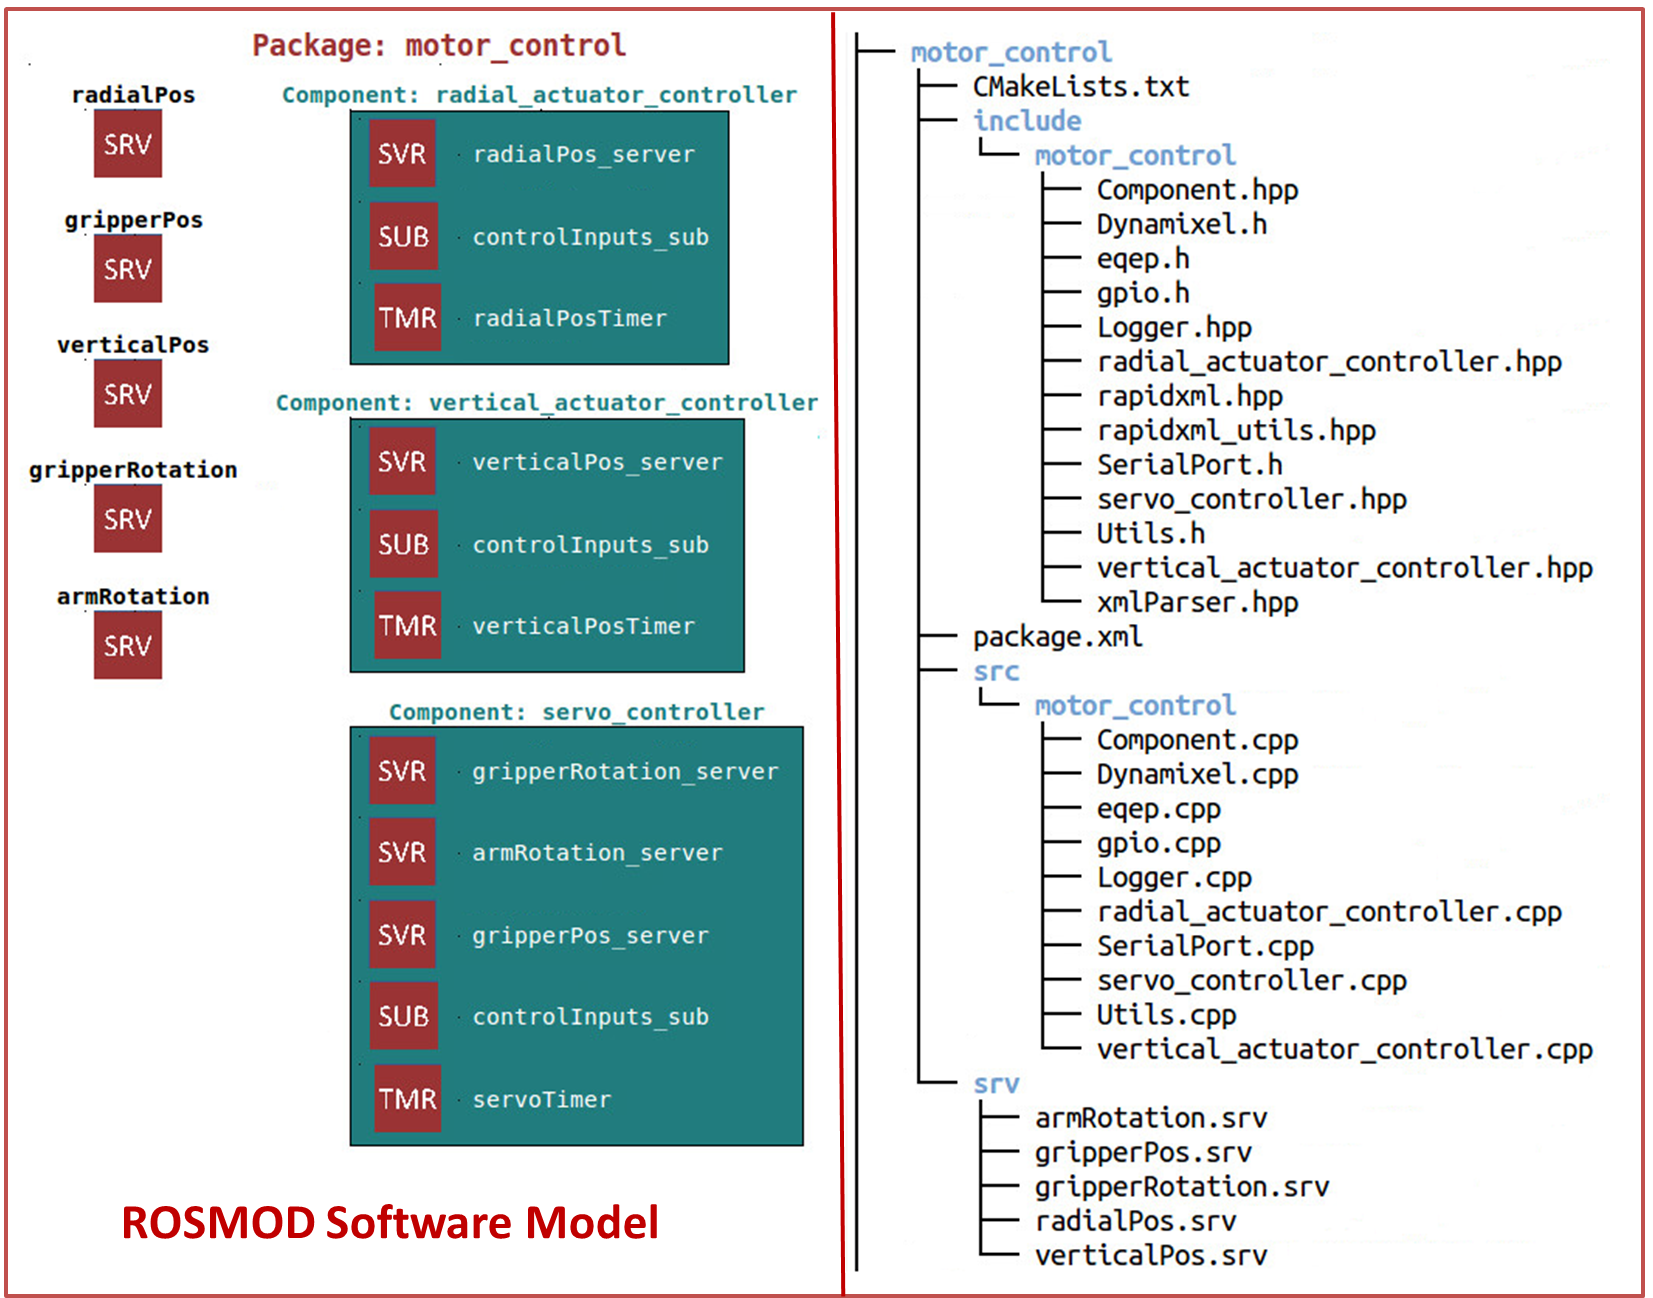
\includegraphics[width=0.50\textwidth]{figs/Code_Generation.png}
	\caption{Workspace Code Generation}
	\label{fig:Code_Generation}
\end{figure}

 In each package, the generated code includes code preservation markers around all callbacks and build system files so that users can quickly add new pieces of code which are guaranteed to be preserved after regeneration. This means that users can, for example, (1) generate a ROS workspace for a ROSMOD Software model, (2) add \emph{business logic} code in the generated skeleton callbacks, (3) go back to the models and add additional ports to specific ROSMOD components as required, and (4) regenerate the ROS workspace ensuring preservation of business logic code and selective code additions while accounting for the newly introduced ports. Therefore, users do not need to complete the ROSMOD models to begin C++ code development, enabling on-the-fly feature additions to ROS applications.

\subsubsection{Deployment-specific XML files}

The XML generators produce a batch of configuration files per deployment model. These files are fed to the node executable at run-time to easily change its behavior. Deployment-specific XML files contain properties of component instances in each ROS node, as seen in the deployment model in Figure \ref{fig:ROSMOD_Project}. It is typically desired to have knobs to easily tweak component properties e.g. message queue scheduling scheme, logging levels etc. at run-time without having to rebuild the ROS application. 

\subsection{Deployment Infrastructure}
\label{sec:Deployment_Infrastructure}

The workflow for software deployment is as shown Figure \ref{fig:workflow}. Every ROS workspace is generated with an additional \emph{node} package. This builds a generic node executable that can dynamically load libraries. Once the generators generate the ROS workspace and deployment XML files, users complete application development and build their ROS workspace. The build process generates dynamically loadable libraries, one for each component definition along with a single executable corresponding to the generic node package. The generated XML files contain metadata about about all ROS nodes modeled in the ROSMOD Deployment Model. This includes the component instances in each node and the appropriate component libraries to be loaded. Based on the XML file supplied to the node executable, the node will behave as one of the ROS nodes in the model. This allows for a reusable framework where a generic executable (1) loads an XML file, (2) identifies the component instances in the node, (3) finds the necessary component libraries to load and (4) spawns the executor threads bound to each component. 

\begin{figure}[h]
	\centering
	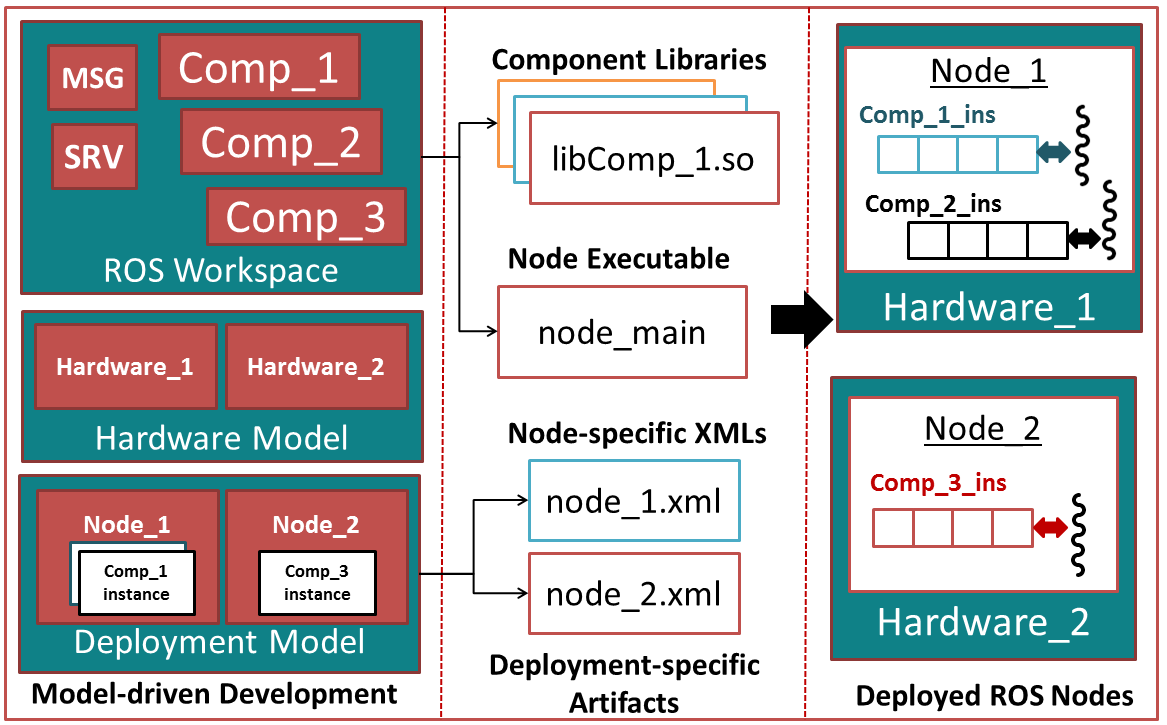
\includegraphics[width=0.50\textwidth]{figs/workflow.png}
	\caption{Software Deployment Workflow}
	\label{fig:workflow}
\end{figure}

In the above architecture, the deployment needs three primary ingredients: (1) the generic node executable, (2) dynamically loadable component libraries, and (3) an XML file for each ROS node in the deployment model. For each new node added to the deployment model, by merely regenerating the XML files, we can establish a new deployment. The ROS workspace is rebuilt only if new component definitions are added to the Software Model. This architecture not only accelerates the development process but also ensures a separation between the Software Model (i.e. the application structure) and deployment-specific concerns e.g. component instantiation inside ROS nodes.

%\subsection{run-time Logging}


%\subsection{Command Line Interface and Testing Framework}

%To automate testing requirements for applications while avoiding graphical strain on low-power embedded devices, ROSMOD also provides a command-line interface. Applications can be developed, built, deployed and managed using just the command line. This enables a testing framework that can be fully automated for large sets of ROSMOD projects as long as the deployment needs are met. This also enables testing a specific ROSMOD project repeatedly and in an automated manner for system-level properties such as timing violations, deadlocks, fault resilience and security requirements.
\section{Case Study: Autonomous Ground Support Equipment}
\label{sec:Case_Study}

This section briefly describes an Autonomous Ground Support Equipment (AGSE) robot that we designed, built, and deployed for the 2014-2015 NASA Student Launch Competition \cite{NASA_SL}. Special emphasis is given to the value of a rapid system prototyping methodology in the design process and how it allowed the AGSE to overcome many of the challenges and problems encountered during the competition.

\subsection{Competition Requirements}

The NASA Student Launch Initiative \cite{NASA_SL} is a research-based competition partnered with NASA's Centennial Challenges in order to stimulate rapid, low-cost development of rocket propulsion and space exploration systems.  Both collegiate and non-academic teams participate in the 8-month competition cycle composed of design, fabrication, and testing of flight vehicles, payloads, and ground support equipment. 

The purpose of the 2014-2015 competition was to simulate a Mars Ascent Vehicle (MAV) and to perform a sample recovery from the Martian surface. The requirements for this simulation were twofold: (1) Design and deploy an AGSE robot that autonomously retrieves a sample off the ground and stores it in the payload bay of a rocket, and (2) launch the rocket to an altitude of 3000 ft. before safely recovering the sample. 

While the driving requirements of the competition were fixed, many of the minor rules regarding AGSE performance, behavior, and safety requirements evolved and were augmented throughout the course of the eight month design cycle. The volatile nature of these rules precipitated the need for rapidly adjustable design and fabrication processes. For this purpose, the mechanical design of the AGSE followed a modular, quick-to-build approach and ROSMOD was used for software development in order to quickly make on-the-fly adjustments to system behavior.

\subsection{Mechanical Design}

The AGSE is a 4-DOF robot utilizing a revolute base joint to rotate the robot body, two prismatic joints to move vertically and horizontally, and a final revolute joint providing an orientation wrist for the end effector to orient a gripper. A wireframe and workspace rendering of the AGSE can be seen in Figure \ref{fig:Render}.

\begin{figure}[h]
	\centering
	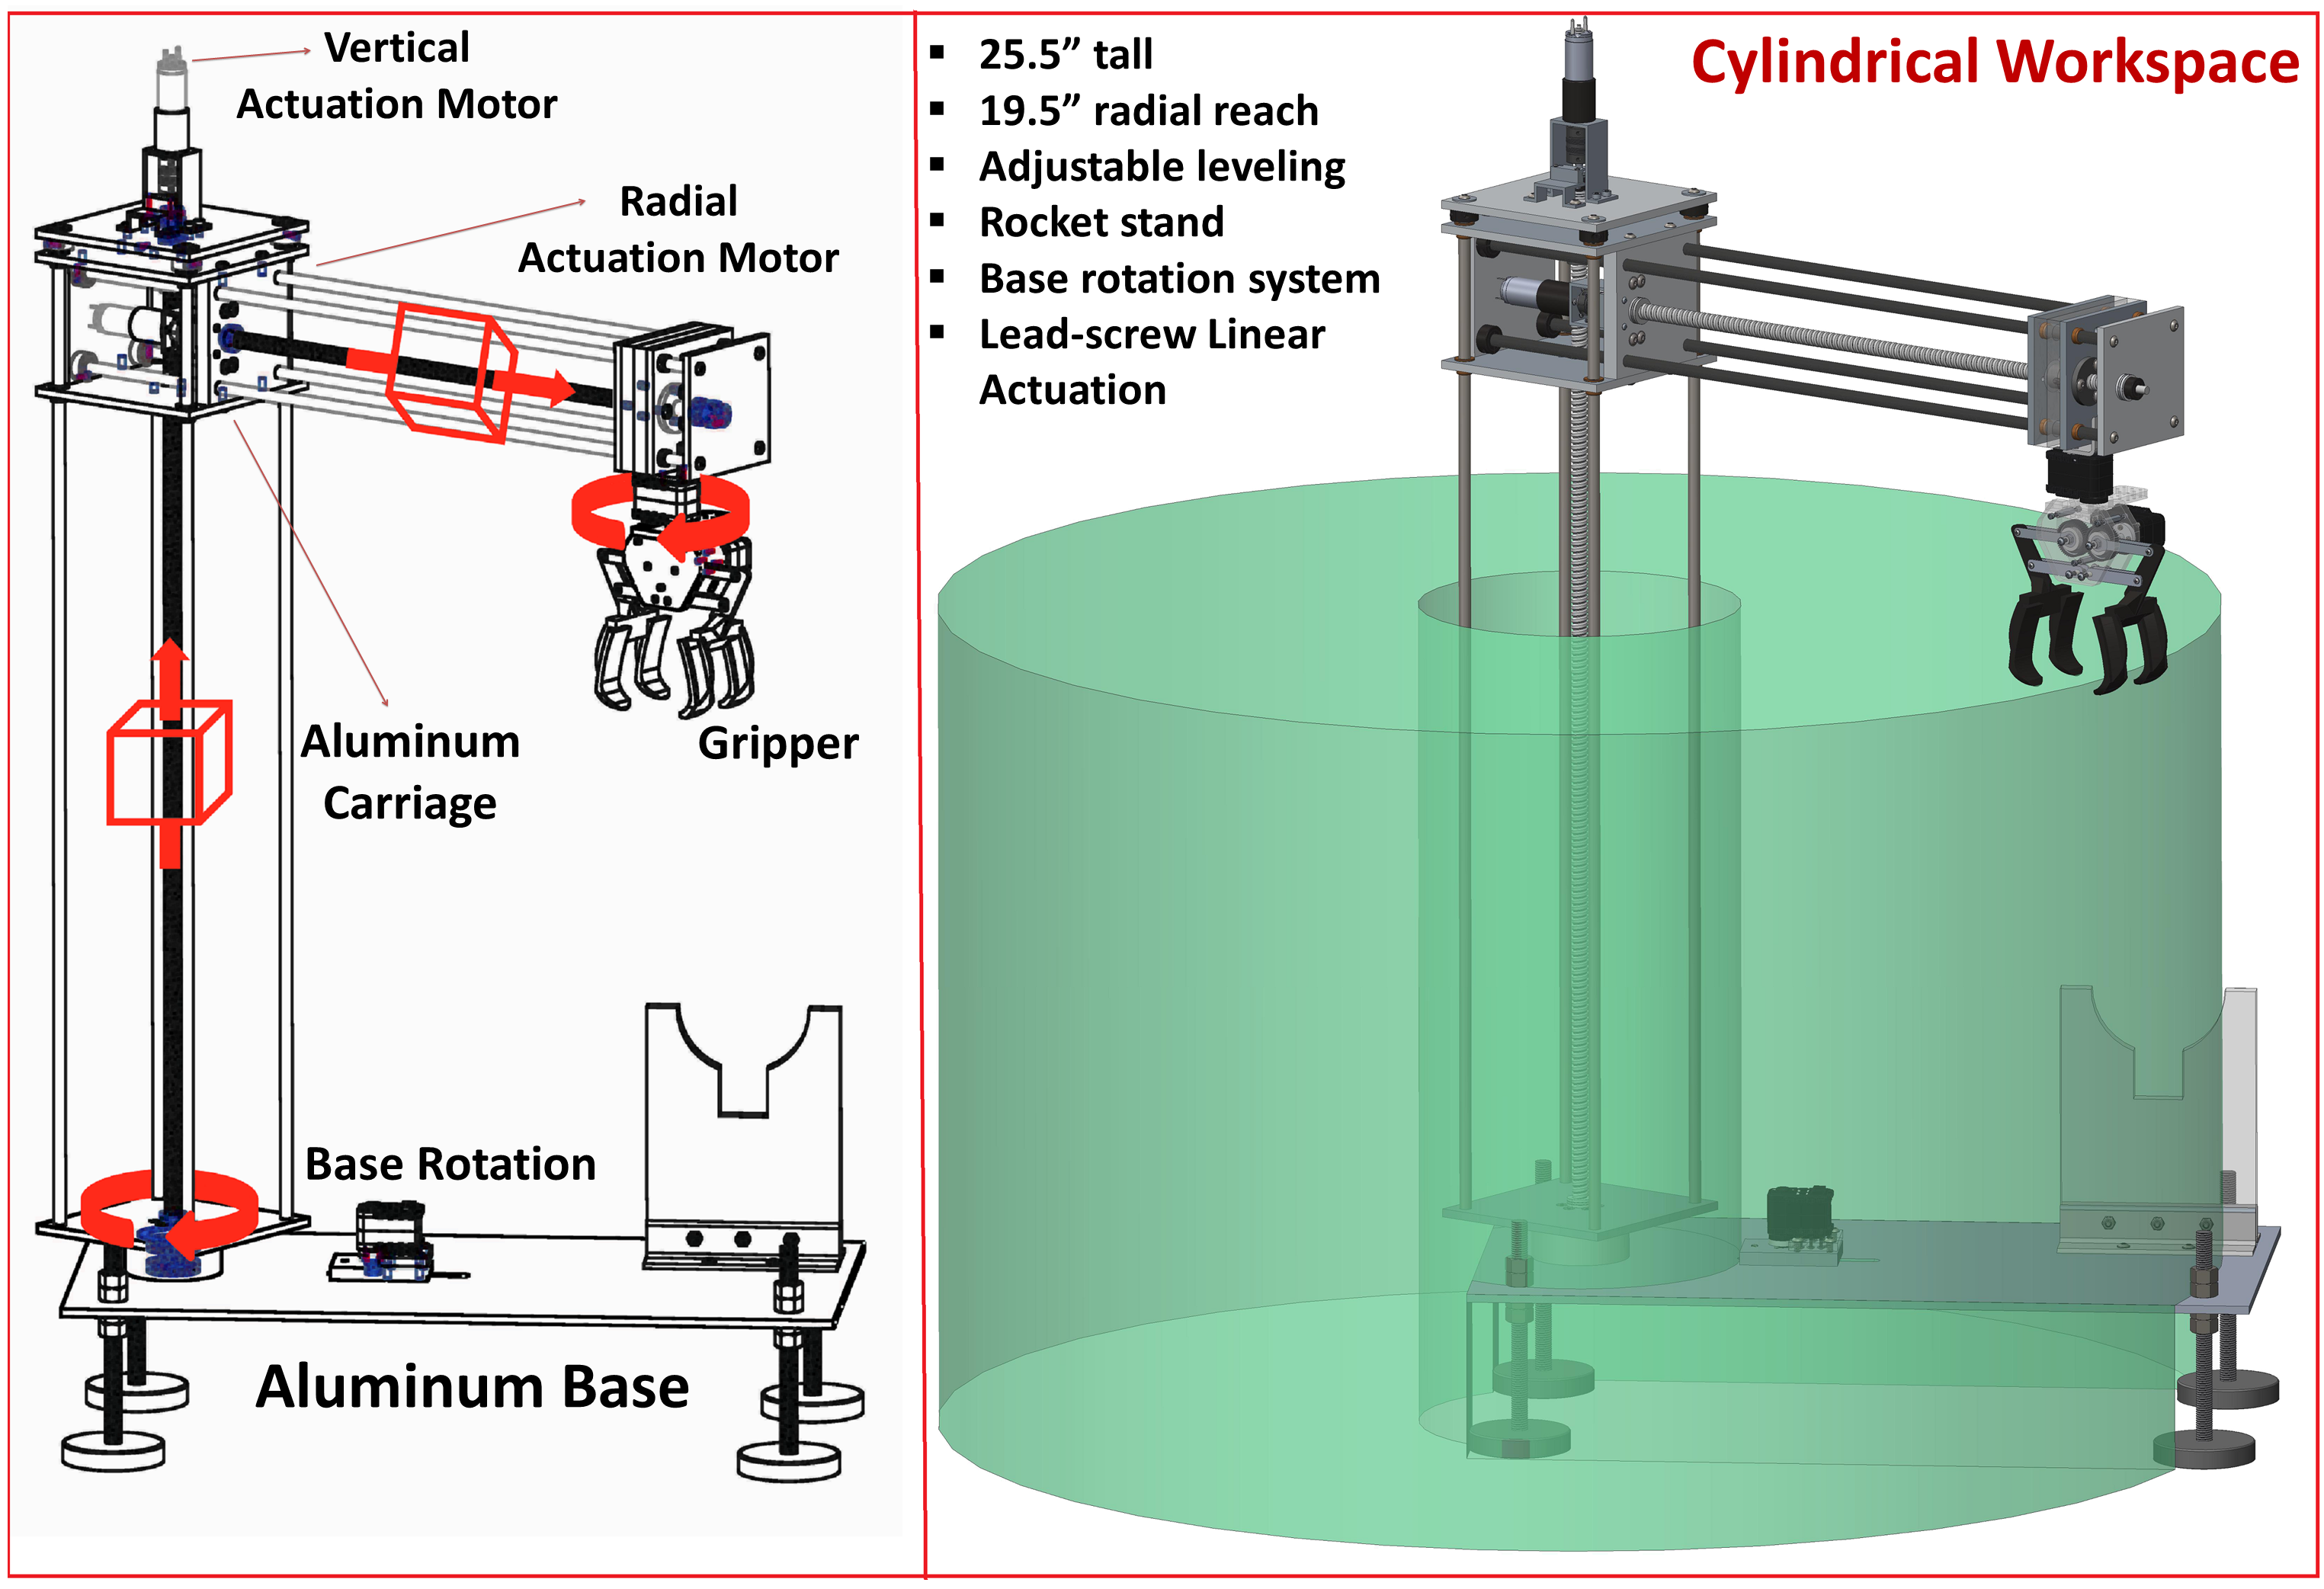
\includegraphics[width=0.48\textwidth]{figs/AGSE_Mechanical_Design_Figure.png}
	\caption{AGSE Mechanical Design}
	\label{fig:Render}
\end{figure}

The AGSE base is comprised of a machined sheet of aluminum, offering a secure mounting point for the upper robotic segments. Above this foundation level, a vertical lead screw, powered by a top-mounted DC motor, drives an aluminum carriage assembly up and down the central rotational axis. A similar lead screw-carriage assembly extends from the side of the vertical carriage to provide motion within the horizontal plane. The combined motion of these joints produces an open-cylindrical workspace. The radially actuating carriage connects to the end effector gripper via a wrist servo motor, which allows the AGSE to interact with the payload and rocket bay.

%The AGSE guides the end effector motion using the limit switch-encoder combo on its linear actuators, the built in positional feedback from the servo motors, and the optical feedback provided by a camera mounted above the end effector (allowing the AGSE to recognize objects within the reachable area underneath the gripper phalanges).

 %The AGSE base is comprised of a machined sheet of aluminum that offers a secure mounting point for the upper robotic segments, majority of the electronics, and the battery pack. Coincident with the base is the first revolute joint. This joint is operated by a servo motor directly coupled to the rotational axis. 
 
 %Vertical movement of the carriage is performed with respect to a limit switch (used to provide a zero reference position) located at the extreme upper limit of travel, and then tracked using an optical encoder to count revolutions of the lead screw.   

One significant set of challenges to the construction of the AGSE were time, machinist skill level, and the facilities available to the group's workforce. The team consisted mainly of undergraduate workers with limited machining experience and no access to CNC machinery.  Due to this constraint, the mechanical design and software needed to accommodate generous tolerance allowances in component machining. The system also needed to be robust enough to recover from the failure of a component, such as that detailed in Performance Assessment.

The short eight month duration of the design cycle, from initial planning to evaluation, meant that the AGSE system had to undergo rapid development.  As such, an iterative, modular, design-build-test approach was implemented in order to concurrently develop as many components of the hardware and software systems as possible. An initial AGSE prototype was conceptualized from off-the-shelf components and the mechanical and software systems were built in parallel, integrated, and tested. These preliminary results were then used in future development to produce a more ideal structure with greater positional accuracy and system robustness.  Due to the modular nature of the system's design, it was not necessary to immediately build a completely new second system, so incremental improvements could be made on a specific subsystem (such as the robot's gripper, any single degree of freedom, image processing, motor control, etc.) as the design evolved.
%\subsection{Image Processing}

%Periodic sample detection performed by the AGSE uses OpenCV-based image processing algorithms to identify and track the sample in real-time. An Image Processor component periodically fetches the latest feed from the mounted camera and performs a series of filtering tasks. 

%Each \emph{RGB} image frame is converted to both \emph{HSV} (hue-saturation-value) and \emph{Grayscale} image frames. After applying thresholds, filters, erosion and dilation methods, the target sample is extracted from the webcam feed. Once the target sample is detected, we draw contours around the object and identify its relative position and orientation. Figures \ref{fig:Sample_Image_Processing} and \ref{fig:Sample_Image_Processing_2} present our launch-day results. 

\subsection{Distributed Deployment}

The AGSE robot is controlled by a distributed set of embedded controllers. Figure \ref{fig:AGSE_Deployment} shows the high-level design for the deployment architecture. There are three embedded devices, each with its own responsibilities. 

\begin{figure*}[t]
	\centering	
	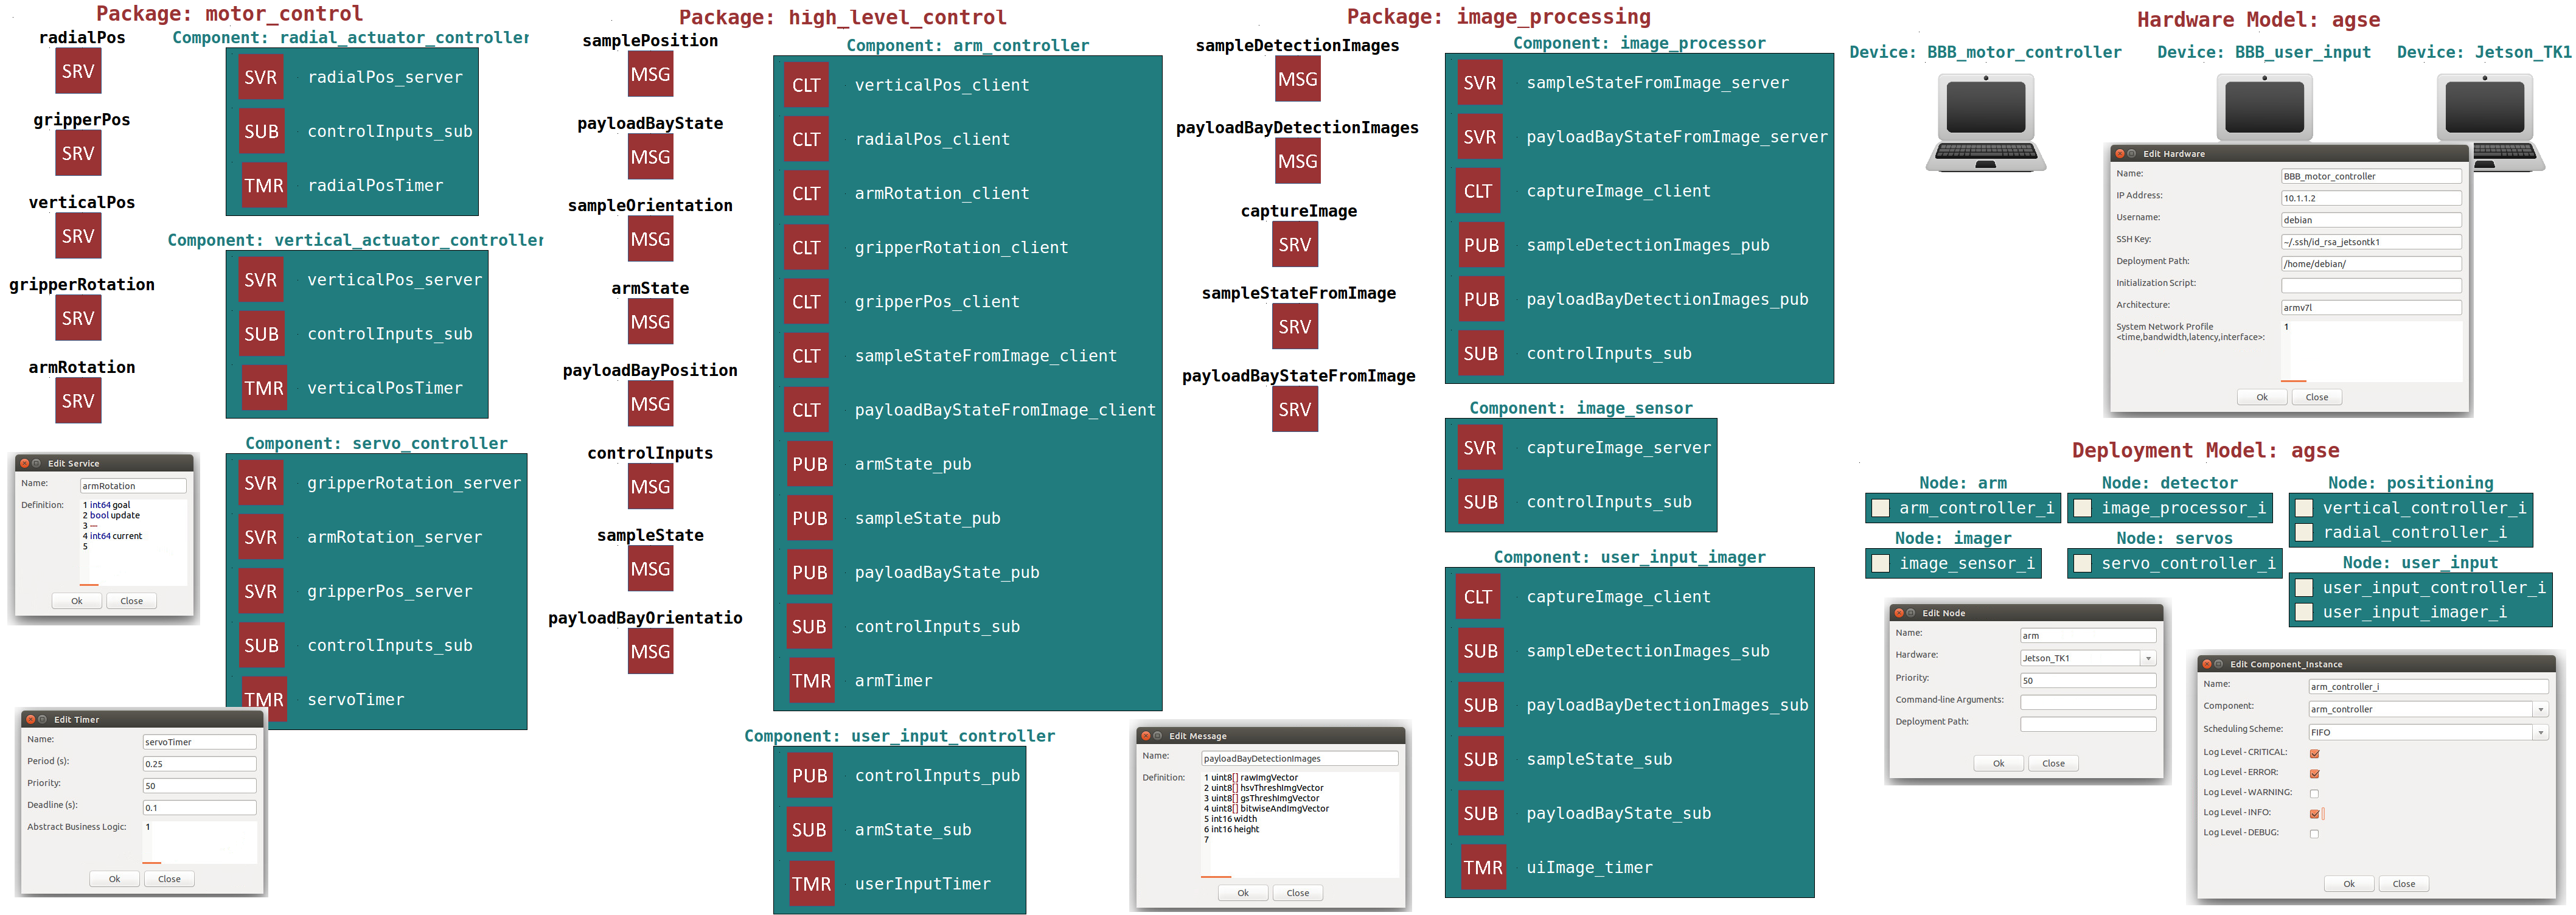
\includegraphics[width=1.0\linewidth]{figs/AGSE.png}
	\caption{AGSE ROSMOD Model}
	\label{fig:AGSE}	
\end{figure*}


An NVIDIA Jetson TK1 periodically fetches the latest webcam feed, performs image processing and high-level path planning, updating a global state machine. A Beaglebone black (BBB) mounted on top of the robot performs power management, low-level motor control and feedback processing. Lastly, a \emph{User Input Panel} houses a second Beaglebone Black, reacting to user input e.g. pause switch, touchscreen mode changes etc. This last controller is also responsible for keeping the user informed about the real-time state of the AGSE and the current webcam feed. Each of these controllers host ROS multiple nodes with ROSMOD component executor threads periodically performing algorithmic computations, calculating new robotic paths and maintaining the global state machine.

\begin{figure}[h]
	\centering
	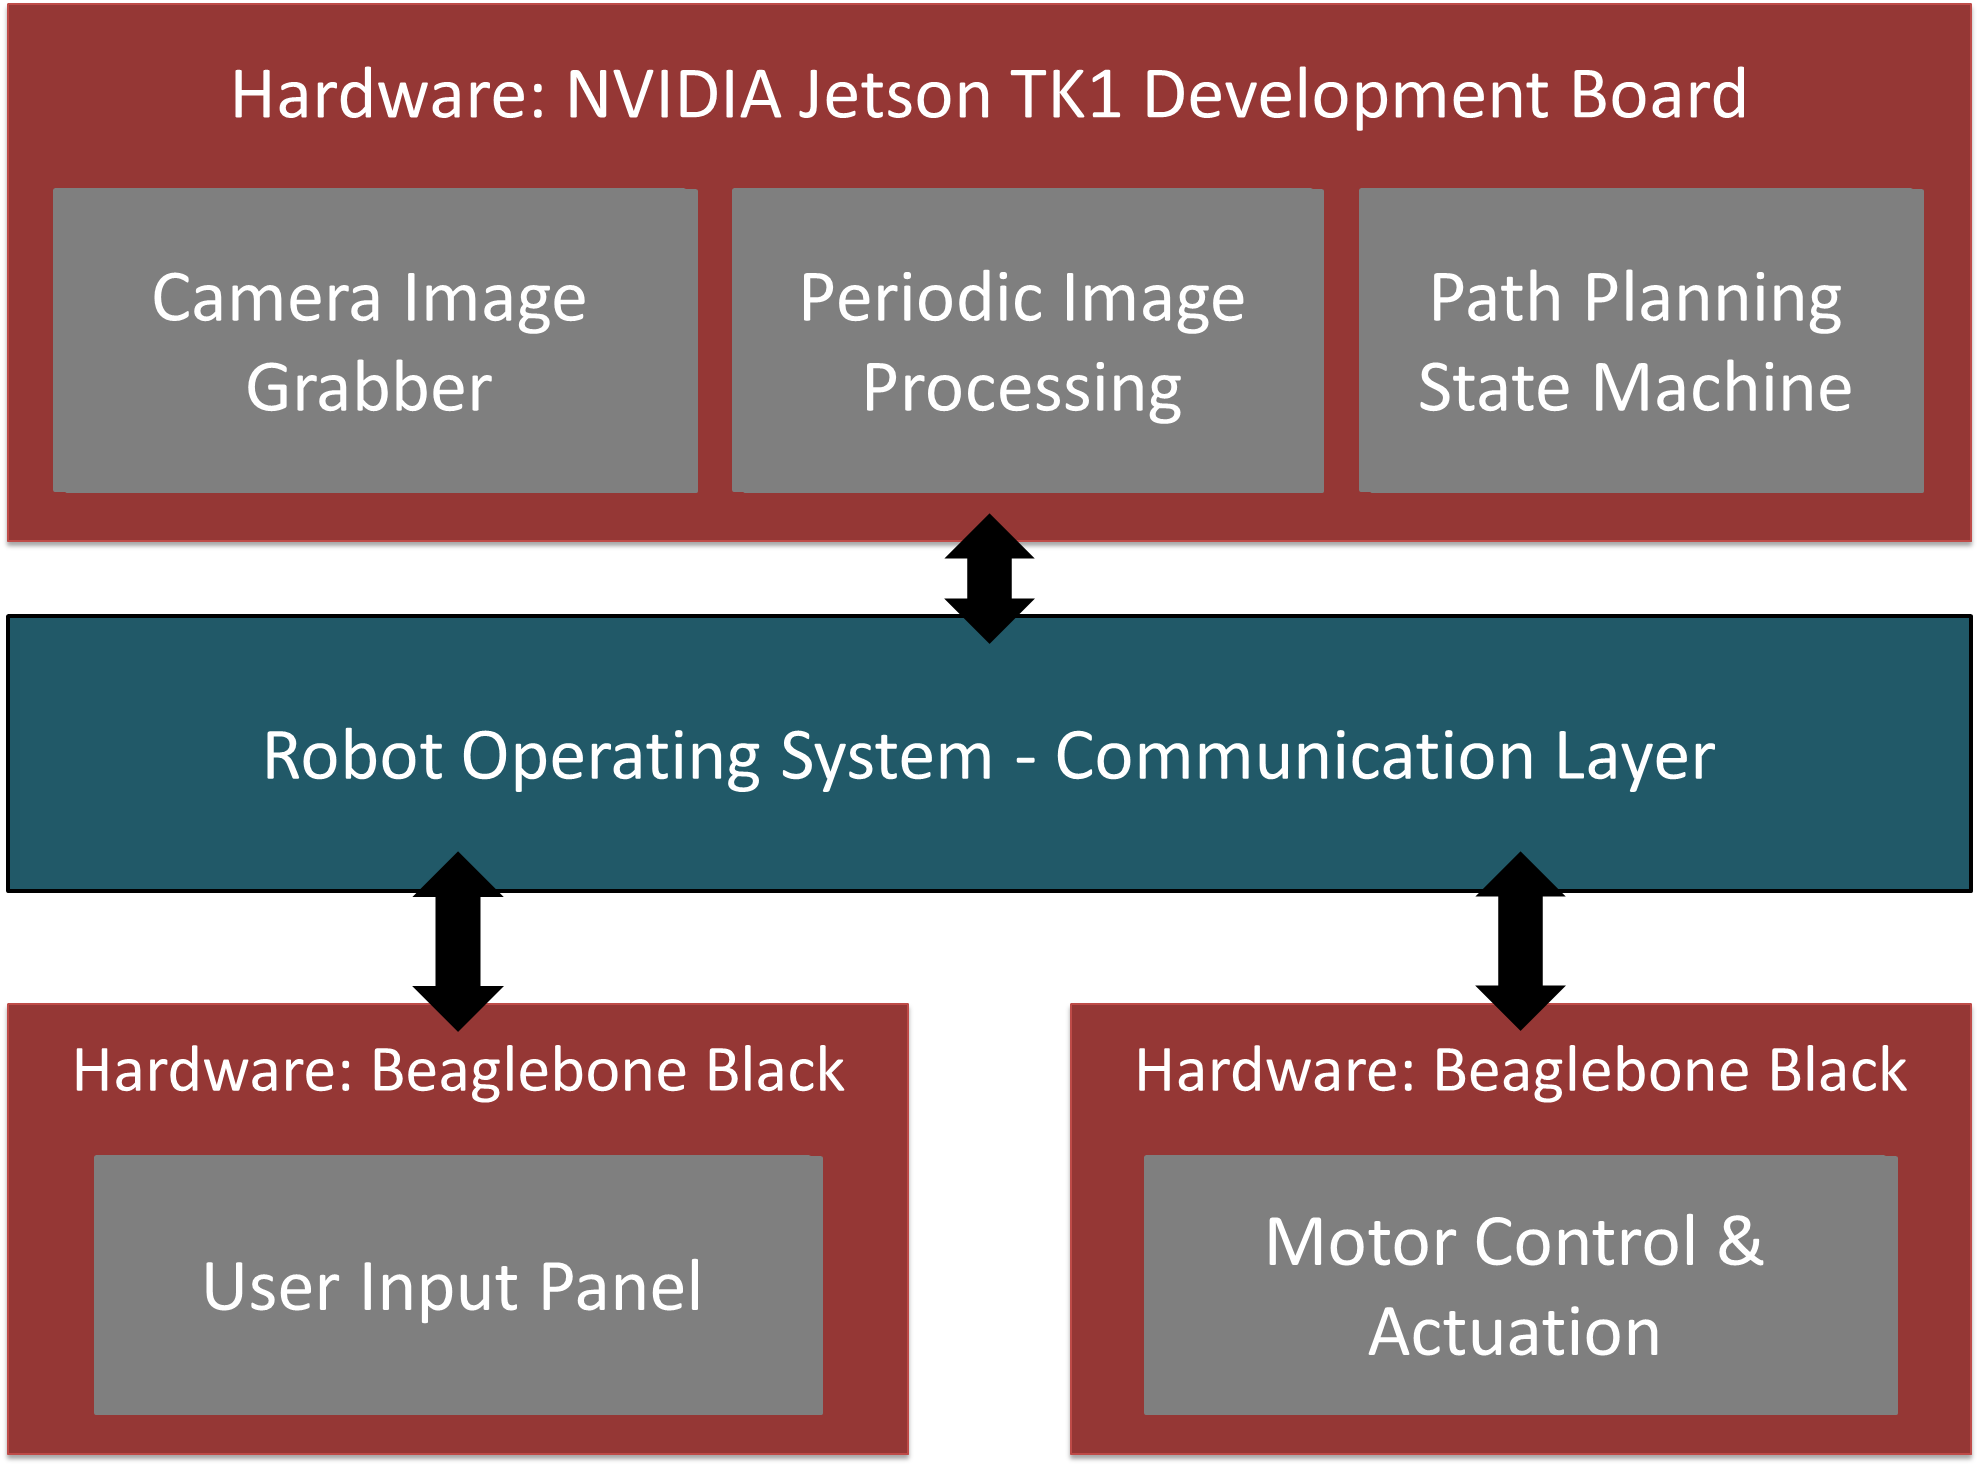
\includegraphics[width=0.45\textwidth]{figs/AGSE_Deployment.png}
	\caption{AGSE Package Deployment}
	\label{fig:AGSE_Deployment}
\end{figure}

\subsection{Software Prototyping with ROSMOD}

The AGSE software \cite{AGSE} was iteratively designed and rapid prototyped using ROSMOD. Figure \ref{fig:AGSE} shows the fully constructed ROSMOD models for the AGSE. The Software Model consists of 8 components spread across three ROS packages - motor control, high-level state machine control and image processing. Each package is characterized by its local set of messages, services and interacting components. 

The deployment model shows the various ROS nodes in the final system. Each node instantiates one or more components defined in the Software model e.g. the \emph{positioning} node executes two component threads, one behaving as a vertical\_actuator\_controller component and the other behaving as a radial\_actuator\_controller component. Each of these nodes is then deployed on one of the hardware devices modeled in the hardware model.

The ROSMOD code generators enabled generation of nearly 60\% (6,000+ lines) of the total built code. For systems like the AGSE with a medium-to-large set of interacting components, a small change to the message structure, port coupling, or functional dependencies can require a cascading and exponentially increased set of code changes. Typically, without ROSMOD, such code-breaking changes can cause a few days of work to fix and the build system can become brittle. This process can be cumbersome and error prone, especially when structural changes to software are frequent.

However, using ROSMOD's code generation and preservation features, such changes can be countered with a few seconds of code regeneration. As developers, we had to fill in the missing pieces - the business logic of the generated callbacks, completing the component interaction loops. This code includes architecture-specific control, e.g. GPIO and encoder readings, LED and switch settings, camera image acquisition, and high-level control. Although the overall software was frequently redesigned and tweaked, a large portion of this code required at most a few weeks of development and testing - a time frame that would not have been met without ROSMOD. 

\subsection{Performance Assessment}

At the competition, the Vanderbilt AGSE was able to complete the sample retrieval process in approximately $4.5$ minutes. The recovery process, as shown in Figure \ref{fig:AGSE_Operation}, was successful, with payload and rocket bay recognition occurring quickly and efficiently. The AGSE was able to grasp the payload using only two of its four padded end effector phalanges, and successfully deposited the payload within the rocket bay. This operation received high marks from the NASA officials and earned the competition's \emph{Autonomous Ground Support Equipment Award}.

System robustness was validated on the day of competition when a key component failed and was able to be quickly replaced with a different part with no detriment to system performance. The Dynamixel AX-12A servo controlling the base rotational degree of freedom of the AGSE suffered an irreparable failure of its gearbox and had to be removed from the robot. A backup of the servo was not readily available, and a different model servo by the same company had to be swapped in instead.  This new model, a Dynamixel MX-28T, while having similar performance as the old servo, had a different communication protocol and mounting footprint, as well as a more complex control scheme.

The component-based nature of ROSMOD allowed quick modifications of the business logic of the \emph{servo\_controller} package to update the system to use the new hardware.  The new control scheme was quickly implemented and the new physical placement of the servo due to its different mounting footprint was accounted for in software. After these modifications were made, the AGSE was able to perform at its optimal level during its part of the competition.

The rapid prototyping facilitated by ROSMOD and the ROS infrastructure enabled the development of an overall \emph{smarter} robot. The software requirements for autonomy were matched by the ROSMOD code generators such that developers had to spend little time setting up the build system and interaction patterns. The speed of development was drastically improved and the \emph{business logic} code, i.e. the core of the implementation of the system behavior, could be made more robust.


\begin{figure}[h]
	\centering	
	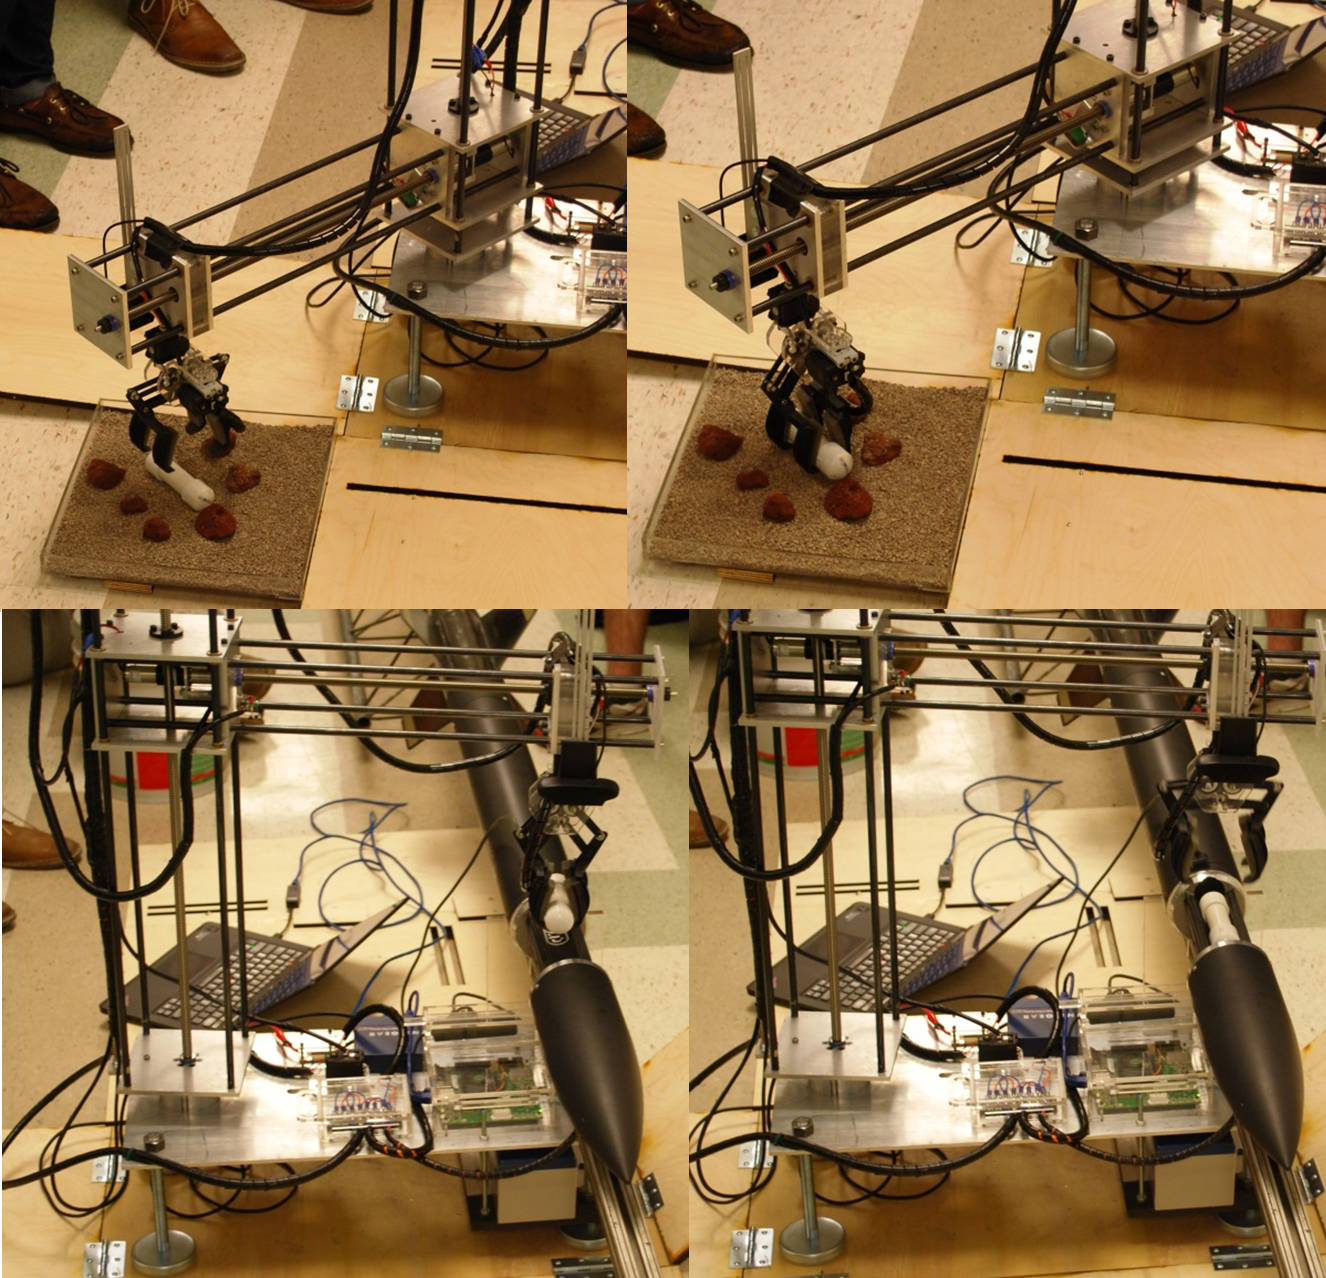
\includegraphics[width=1.0\linewidth]{figs/AGSE_Operation.png}
	\caption{AGSE Calibration and Testing}
	\label{fig:AGSE_Operation}	
\end{figure}
\vspace{-0.1in}


\section{Future Work}
\label{sec:Future_Work}

% Analysis tools
Building robust, stable and deterministic applications using ROSMOD requires both design-time analysis and runtime management with potential reconfiguration solutions. Our previous work on timing analysis \cite{MoDeVVa}\cite{SEUS} and network QoS analysis \cite{ISIS_F6_CYPHY:14} for component-based distributed real-time systems has given us good insight into the verification and validation requirements, challenges and general design principles for such systems. Since these methods are model-based and generic, we plan to completely integrate these tools into ROSMOD such that any deployment model can be studied at design-time for potential timing anomalies and network capacity and admittance issues. 

To facilitate this, current work on the ROSMOD runtime package aims at introducing deadline monitoring on a per-component basis. The goal of this monitoring thread is to detect deadline violations in all callbacks and operations handled by the component executor thread. This helps in identifying inefficient priority assignments and schedule feasibility issues, which are typical demands for mission-critical real-time systems.


\section{Related Research}

Developing resilient software for CPS presents a unique challenge. These systems execute software pieces that are often times distributed across a collection of machines, presenting risks and challenges to both human safety and developmental costs. Research in such areas require tools and testbeds that enable an approximated evaluation of the real system. As a widely acknowledged challenge, several testbed architectures have been proposed in the past tackling heterogeneous concerns in CPS design such as security, fault tolerance and determinism. 

Among the various application design challenges, many testbeds have focused on security research for CPS. Often, the interactions between hardware components and software control code in the real system is hard to replicate for testing, mainly in dynamic real-world-like environments. For example, in automotive networks, although the networking methods are standards like CAN, the implementation details are left to the hands of the board manufacturers and not easily accessible. 

The maintainers of OCTANE \cite{OCTANE} tackle these issues by providing a software package and a hardware infrastructure to reverse engineer and test automotive networks. By replicating the interactions between the system hardware and the control software, users can focus on security aspects in such networks instead of configuring and setting up the testing tools.

Similarly, the UPBOT \cite{UPBOT} testbed provides a testbed for cyber-physical systems used primarily to test security threats and preventive measures. It presents a testing infrastructure to study several points of attack on programmable component-based systems where the on-board intelligence may be exhibiting safety-critical properties. The low cost and ease of use makes this an appreciable learning tool for students and researchers, especially ones lacking access to such testing environments. 

In an alternate study, the Pharos \cite{Pharos} testbed provides a testing framework for mobile CPS. Using a networked system of autonomously mobile communicating controllers, the testbed demonstrates its utility in live testing of mobile CPS deployments, with comparisons against system simulation schemes. The study shows the absolute importance of validating simulation results with real-world experimentation and how Pharos enables such testing. 
\section{Conclusions}
\label{sec:Conclusions}

Robot Operating System (ROS) is one of few preferred and widely accepted platforms to develop large-scale robotics applications. ROS provides a light-weight middleware framework and a variety of command-line tools to quickly prototype and execute interacting processes. However, much of the development process with ROS can still be automated and there is a need for development tool suites that are easily accessible and that, using model-driven development principles, can provide for a rich set of design-time features such as modeling, code generation, analysis, deployment and process monitoring along with run-time support for general fault management. 

The ROSMOD toolsuite presented in this paper supports all these capabilities, as shown in our case study. However, one of the most important aspects of such development tools is the often neglected support for analysis, which is especially relevant in safety-critical real-time systems. Our current work aims at integrating our existing model-driven analysis tools into ROSMOD to support not only a wider range of systems but also a larger user group.

%We have evaluated the usability of ROSMOD by prototyping a sample recovery robot for the NASA competition. 
 
 

% Acknowledgement
\section*{Acknowledgment}

This work was supported by DARPA under contract NNA11AB14C and USAF/AFRL under Cooperative Agreement FA8750-13-2-0050, and by the National Science Foundation (CNS-1035655). The activities of the 2014-15 Vanderbilt Aerospace Club were sponsored by the Department of Mechanical Engineering and the Boeing Corporation. Any opinions, findings, and conclusions or recommendations expressed in this material are those of the author(s) and do not necessarily reflect the views of DARPA, USAF/AFRL, NSF, or the Boeing Corporation. Lastly, the authors would also like to thank the following undergraduate students on the AGSE design team for their invaluable work: Connor Caldwell, Frederick Folz, Alex Goodman, Christopher Lyne, Jacob Moore and Cameron Ridgewell.




\bibliographystyle{IEEEtran}
\bibliography{rosmod}

\end{document}
